%! alt The set of midpoints drawn as a shaded rectangular frame. The outer rectangle RSTU measures 7 by 4, with R at (10, 5) and T at (17, 9), and the unshaded inner rectangle EFGH measures 3 by 2, with E at (12, 6) and G at (15, 8).
%! after_paragraph 3
%! scale 15/14
% The shared preamble of every Cevian figure. pipeline/figures turns these colours into theme-aware paint,
% and refuses any other colour, so draw only with them:
%   figink (lines and labels), figaux (construction lines), figaccent (the object the argument turns on),
%   figtint and figaccenttint (light fills).
\documentclass[border=1.5pt]{standalone}
\usepackage{tkz-euclide}
\definecolor{figink}{RGB}{0,0,0}
\definecolor{figaux}{RGB}{85,85,85}
\definecolor{figaccent}{RGB}{192,57,43}
\definecolor{figtint}{RGB}{221,221,221}
\definecolor{figaccenttint}{RGB}{245,213,208}
% tkz-euclide's defaults draw circles, compasses and marks in 50% grey and fill points with a tint.
\makeatletter
\def\tkz@otherlinecolor{figink}
\def\tkz@euc@circlecolor{figink}
\def\tkz@euc@compasscolor{figink}
\def\tkz@euc@mkcolor{figink}
\def\tkz@mk@fill{figink}
\def\tkz@euc@pointfillcolor{figink}
\makeatother
\tkzSetUpLine[color=figink,line width=.7pt]
\tkzSetUpArc[color=figink,line width=.7pt]
\tkzSetUpCompass[color=figink,line width=.5pt]
\tkzSetUpPoint[color=figink,fill=figink,size=3.1pt]
\tikzset{
  every picture/.style={line cap=round,line join=round,color=figink},
  circle style/.append style={color=figink,line width=.7pt},
  aux/.style={color=figaux,line width=.45pt,dash pattern=on 2.6pt off 2pt},
  key/.style={color=figaccent,line width=1pt},
  mk/.style={color=figink,line width=.5pt},
  lbl/.style={color=figink,inner sep=2.2pt},
  len/.style={color=figink,inner sep=1.5pt,font=\small},
}

\begin{document}
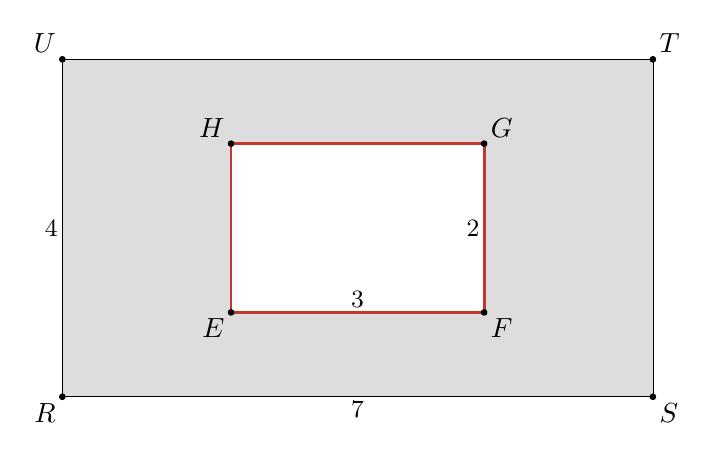
\begin{tikzpicture}
\tkzDefPoint(10.714286,5.3571429){R} %! R = (10, 5)
\tkzDefPoint(18.214286,5.3571429){S} %! S = (17, 5)
\tkzDefPoint(18.214286,9.6428571){T} %! T = (17, 9)
\tkzDefPoint(10.714286,9.6428571){U} %! U = (10, 9)
\tkzDefPoint(12.857143,6.4285714){E} %! E = (12, 6)
\tkzDefPoint(16.071429,6.4285714){F} %! F = (15, 6)
\tkzDefPoint(16.071429,8.5714286){G} %! G = (15, 8)
\tkzDefPoint(12.857143,8.5714286){H} %! H = (12, 8)
%! fact dist(R, S) == 7
%! fact dist(S, T) == 4
%! fact dist(E, F) == 3
%! fact dist(F, G) == 2
%! fact perp(R, S, S, T)
%! fact perp(E, F, F, G)
\tkzFillPolygon[color=figtint](R,S,F,E)
\tkzFillPolygon[color=figtint](S,T,G,F)
\tkzFillPolygon[color=figtint](T,U,H,G)
\tkzFillPolygon[color=figtint](U,R,E,H)
\tkzDrawPolygon(R,S,T,U)
\tkzDrawPolygon[key](E,F,G,H)
\tkzDrawPoints(R,S,T,U,E,F,G,H)
\tkzLabelPoint[below left,lbl](R){$R$}
\tkzLabelPoint[below right,lbl](S){$S$}
\tkzLabelPoint[above right,lbl](T){$T$}
\tkzLabelPoint[above left,lbl](U){$U$}
\tkzLabelPoint[below left,lbl](E){$E$}
\tkzLabelPoint[below right,lbl](F){$F$}
\tkzLabelPoint[above right,lbl](G){$G$}
\tkzLabelPoint[above left,lbl](H){$H$}
\tkzLabelSegment[below,pos=.5,len](R,S){$7$}
\tkzLabelSegment[left,pos=.5,len](U,R){$4$}
\tkzLabelSegment[above,pos=.5,len](E,F){$3$}
\tkzLabelSegment[left,pos=.5,len](F,G){$2$}
\end{tikzpicture}
\end{document}
